\documentclass{article}

\usepackage{graphicx} % Required for inserting images
\usepackage[slovene]{babel}
\usepackage{gensymb}
\usepackage{titling}
\usepackage{arydshln} % za črtkane črte v tabelah(\hdashline)
\usepackage{subfigure}

\title{3. domača naloga}
\author{Tine Zaletelj}
\date{\today}

\begin{document}
\maketitle

\section{Povzetek naloge}
Obravnavali smo delec z nabojem e=1 v zunanjem magnetnem polju $B=B_0$ v smeri z-osi. Delec je pripet na prožno vzmet in se giba v ravnini xy. Na začetku ga izmaknemo iz ravnovesne lege na položaj $r_0=(0.2, 0)$, pri čemer velja $v_0=0.$ Delec nato spustimo da zaniha, kot to opisuje diferencialna enačba (\ref{en}). Pri nalogi smo za konstanto vzmeti vzeli vrednost k=1. V prvem delu naloge smo narisali premikanje delca za 3 različne vrednosti $B_0 = 0.1; 1; 10.$ Rezultate prikazuje slika \ref{fig:enter-label1}.

V drugem delu naloge smo narisali graf minimalne razdalje od izhodišča v odvisnosti od jakosti zunanjega magnetnega polja $B_0$. Ugotovili smo, da močnejše kot je polje, bolj se gibanje delca približuje krožnici. Rezultate prikazuje slika \ref{2}

\begin{equation}
    m\frac{d^2r}{dt^2} = -k\frac{|r|-r_0}{|r|}r + e\frac{dr}{dt}\times B
    \label{en}
\end{equation}

\begin{figure}
    \centering
    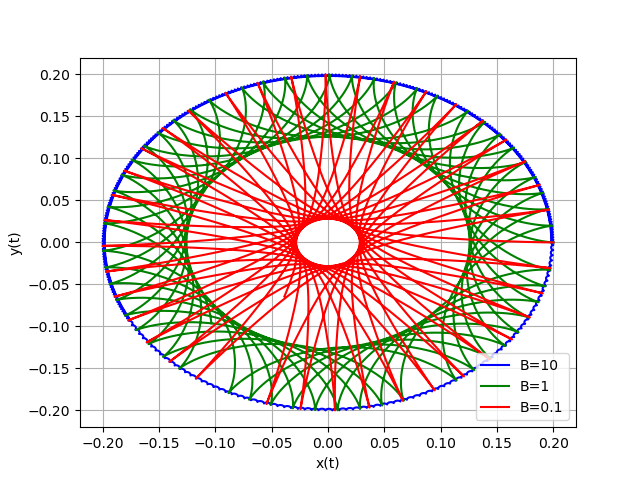
\includegraphics[width=8cm]{slika1.png}
    \caption{Gibanje delca v ravnini xy pri treh različnih vrednostih $B_0$}
    \label{fig:enter-label1}
\end{figure}

\begin{figure}
    \centering
    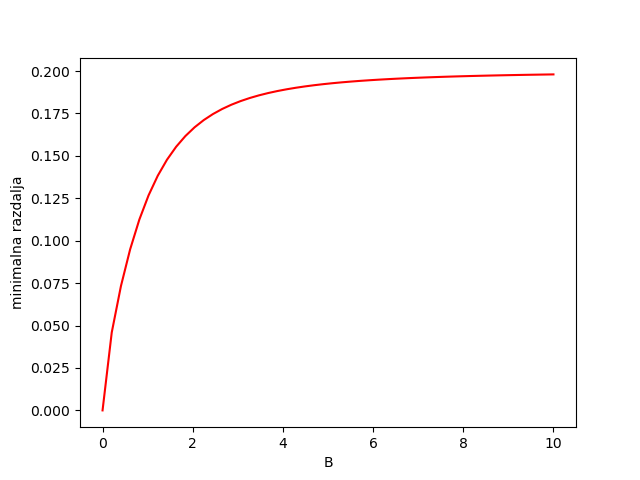
\includegraphics[width = 8cm]{slika2.png}
    \caption{Minimalna razdalja od izhodišča v odvisnosti od jakosti zunanjega magnetnega polja $B_0$}
    \label{2}
\end{figure}


\end{document}
